\documentclass{beamer}
\usetheme{Madrid}
\usecolortheme{beaver}
\graphicspath{{../figures/}{../}}

\title[GA for TSP]{Genetic Algorithm for the Travelling Salesman Problem}
\subtitle{A study on 15 Indian cities, validated against the exact optimum}
\author[Shashwat Shikhar Dwivedi]{Shashwat Shikhar Dwivedi\\Roll No.\ 2427030605}
\institute[CSE]{Department of Computer Science and Engineering\\
Artificial Intelligence and Soft Computing (CSE3121)\\
Submitted to: Dr.\ Neha Chaudhary}
\date[2026--27]{Academic Year 2026--27}

\AtBeginSection[]
{
  \begin{frame}
    \frametitle{Outline}
    \tableofcontents[currentsection]
  \end{frame}
}

\begin{document}

\frame{\titlepage}

\begin{frame}
\frametitle{Outline}
\tableofcontents
\end{frame}

\section{Problem and Approach}

\begin{frame}
\frametitle{The Travelling Salesman Problem}
Visit each of 15 Indian cities exactly once and return to the start, minimising total distance.
\[
  L(\pi)=\sum_{i=1}^{n} d\bigl(\pi_i,\pi_{(i \bmod n)+1}\bigr)
\]
\begin{itemize}
 \item $(15-1)!/2 \approx 4.4\times10^{10}$ distinct tours
 \item NP-hard, so brute force is impractical
 \item Distances: great-circle (haversine) between city coordinates
\end{itemize}
\end{frame}

\begin{frame}
\frametitle{Why a Genetic Algorithm?}
\begin{itemize}
 \item Population-based search inspired by natural selection
 \item Explores many regions of the search space in parallel
 \item Recombination combines good partial routes from different tours
\end{itemize}
\vspace{0.5em}
\begin{alertblock}{Objectives}
Implement a GA from scratch, validate it against the exact optimum (Held--Karp), compare with baselines, and study mutation rate and population size.
\end{alertblock}
\end{frame}

\section{GA Design}

\begin{frame}
\frametitle{GA Design}
\begin{tabular}{ll}
\textbf{Component} & \textbf{Choice} \\ \hline
Chromosome & Permutation of city indices \\
Fitness & $1/L(\pi)$ \\
Selection & Tournament, $k=5$ \\
Crossover & Order Crossover (OX1), prob.\ 0.9 \\
Mutation & Segment inversion, prob.\ 0.2 \\
Elitism & Best 2 copied unchanged \\
Population / generations & 150 / 300 \\
\end{tabular}
\vspace{0.5em}

A permutation encoding means every chromosome is a valid tour.
\end{frame}

\begin{frame}
\frametitle{Worked Example: Order Crossover}
\begin{columns}
\column{0.55\textwidth}
Parents (8 cities), slice at positions 2--4:
\begin{itemize}
 \item P1 = [1, 2, \alert{3, 4, 5}, 6, 7, 8]
 \item P2 = [3, 7, 5, 1, 6, 8, 2, 4]
\end{itemize}
Keep \alert{[3, 4, 5]} from P1, fill the rest in P2 order: 7, 1, 6, 8, 2.
\column{0.45\textwidth}
\begin{block}{Child}
[7, 1, \alert{3, 4, 5}, 6, 8, 2]
\end{block}
\begin{block}{Inversion mutation}
[1, 2, 3, 4, 5, 6, 7, 8] $\to$ [1, 2, \alert{6, 5, 4, 3}, 7, 8]
\end{block}
\end{columns}
\end{frame}

\section{Results}

\begin{frame}
\frametitle{Exact Optimum vs.\ GA Tour}
\begin{columns}
\column{0.5\textwidth}
\centering
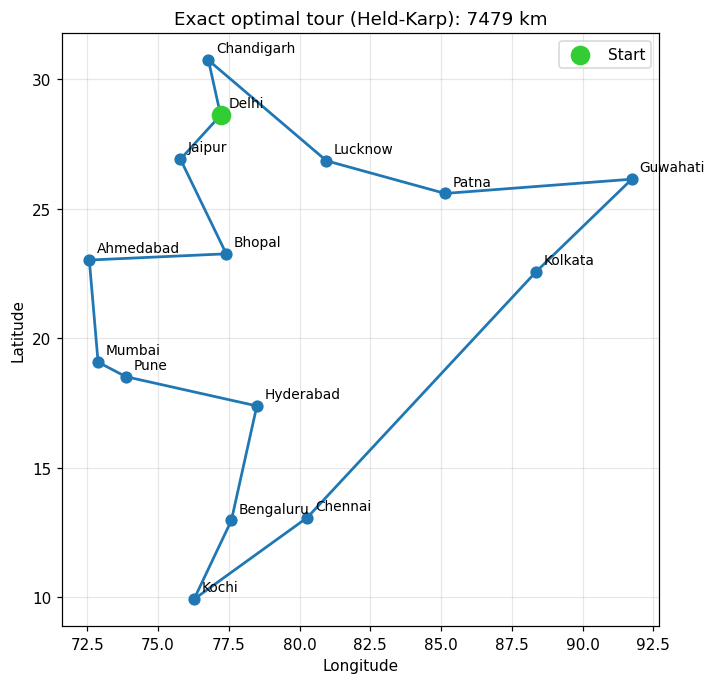
\includegraphics[height=0.62\textheight]{optimal_route.png}\\
{\small Held--Karp: 7478.9 km}
\column{0.5\textwidth}
\centering
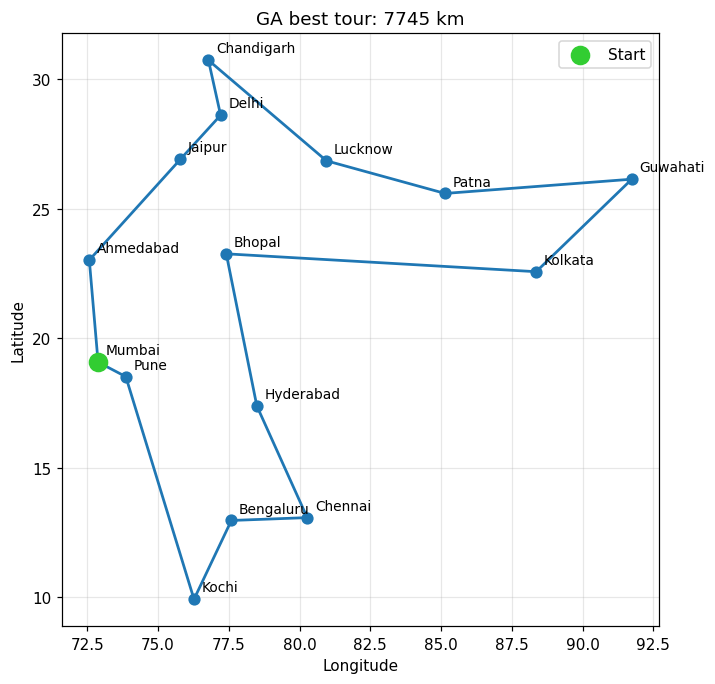
\includegraphics[height=0.62\textheight]{ga_route.png}\\
{\small GA, one run (seed 42): 7745.4 km}
\end{columns}
\end{frame}

\begin{frame}
\frametitle{Convergence}
\centering
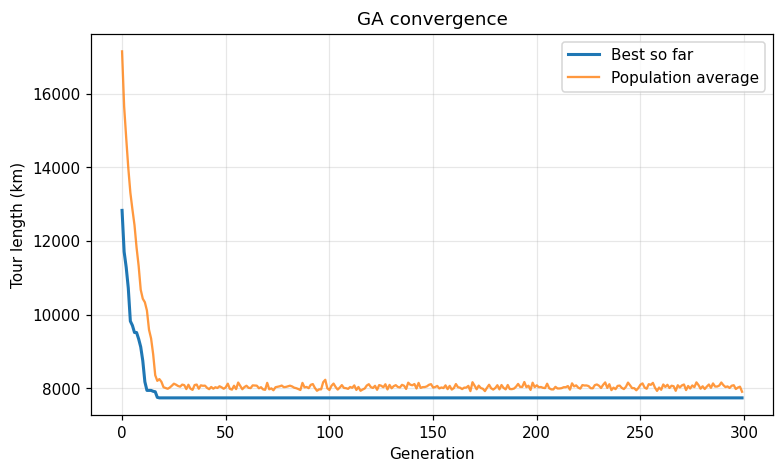
\includegraphics[height=0.68\textheight]{ga_convergence.png}

The best tour improves quickly while the population average follows.
\end{frame}

\begin{frame}
\frametitle{GA versus Baselines}
\begin{center}
\begin{tabular}{lrr}
\textbf{Method} & \textbf{Length (km)} & \textbf{Gap (\%)} \\ \hline
Random search (same budget) & 9930.4 & 32.8 \\
Nearest neighbour & 9169.4 & 22.6 \\
GA (mean of 10 runs) & 7526.9 & 0.6 \\
GA (best of 10 runs) & 7478.9 & 0.0 \\
Exact optimum (Held--Karp) & 7478.9 & 0.0 \\
\end{tabular}
\end{center}
\begin{alertblock}{Key result}
The GA found the true optimum in 5 of 10 runs, and averaged 0.6\% above optimal.
\end{alertblock}
\end{frame}

\begin{frame}
\frametitle{Effect of Mutation Rate}
\begin{columns}
\column{0.52\textwidth}
\centering
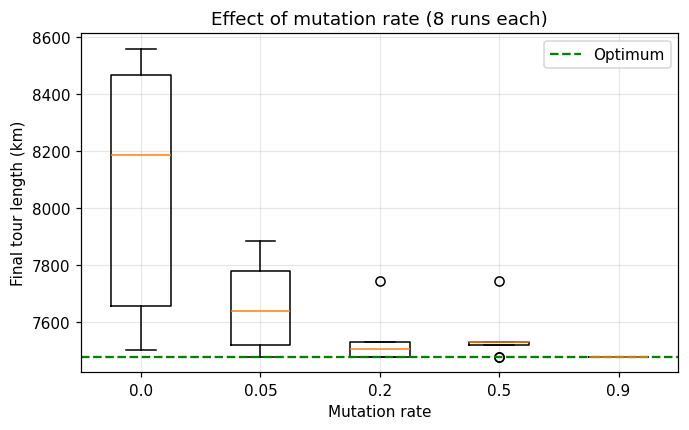
\includegraphics[width=\textwidth]{mutation_rate.png}
\column{0.48\textwidth}
\begin{tabular}{rr}
\textbf{Rate} & \textbf{Mean (km)} \\ \hline
0.00 & 8079.0 \\
0.05 & 7660.8 \\
0.20 & 7532.2 \\
0.50 & 7545.6 \\
0.90 & 7478.9 \\
\end{tabular}
\vspace{0.5em}

{\small No mutation performs worst: it stagnates.}
\end{columns}
\end{frame}

\begin{frame}
\frametitle{Effect of Population Size}
\begin{columns}
\column{0.52\textwidth}
\centering
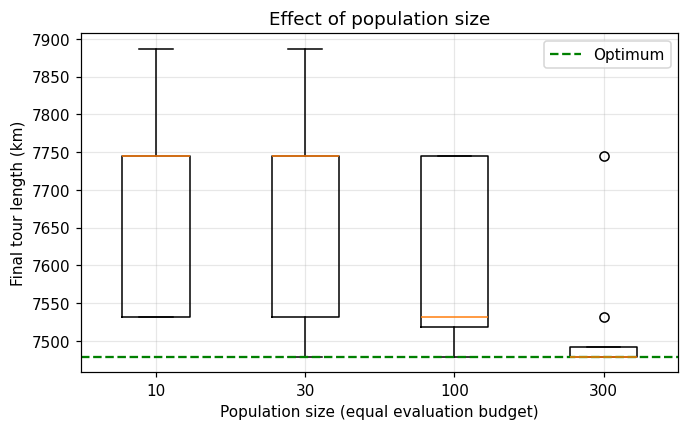
\includegraphics[width=\textwidth]{population_size.png}
\column{0.48\textwidth}
\begin{tabular}{rrr}
\textbf{Pop.} & \textbf{Gens} & \textbf{Mean (km)} \\ \hline
10 & 4500 & 7683.1 \\
30 & 1500 & 7676.5 \\
100 & 450 & 7598.8 \\
300 & 150 & 7518.9 \\
\end{tabular}
\vspace{0.5em}

{\small Equal budget of 45{,}000 evaluations.}
\end{columns}
\end{frame}

\section{Conclusion}

\begin{frame}
\frametitle{Complexity and Limitations}
\begin{itemize}
 \item GA time $O(G\cdot P\cdot n)$, space $O(P\cdot n)$
 \item Held--Karp: $O(n^2 2^n)$ time, $O(n\,2^n)$ space, impractical beyond about 25 cities
 \item No optimality guarantee; results depend on parameters and seed
 \item Premature convergence when diversity is lost (seed 42 ended 3.6\% above optimal)
\end{itemize}
\end{frame}

\begin{frame}
\frametitle{Conclusion}
\begin{itemize}
 \item Within 0.6\% of the exact optimum on average, evaluating only 45{,}000 of $4.4\times10^{10}$ tours
 \item Clearly beats random search (32.8\%) and nearest neighbour (22.6\%)
 \item Mutation prevents stagnation; larger populations win at a fixed budget
 \item Repeated runs are needed because a single run can get stuck
\end{itemize}
\vspace{1em}
\centering \Large Thank you! Questions?
\end{frame}

\end{document}
